\documentclass{article}
% ------------ xcolor ----------- %
\usepackage[usenames,dvipsnames,svgnames,table]{xcolor}
\definecolor{lightgrey}{rgb}{0.96,0.97,0.98}
% if you need to pass options to natbib, use, e.g.:
% \PassOptionsToPackage{numbers, compress}{natbib}
% before loading nips_2016
%
% to avoid loading the natbib package, add option nonatbib:
% \usepackage[nonatbib]{nips_2016}
% to compile a camera-ready version, add the [final] option, e.g.:
% \usepackage[final]{nips_2016}
\usepackage[]{nips_2016}
\usepackage[utf8]{inputenc} % allow utf-8 input
\usepackage[T1]{fontenc}    % use 8-bit T1 fonts
\usepackage{hyperref}       % hyperlinks
\usepackage{url}            % simple URL typesetting
\usepackage{booktabs}       % professional-quality tables
\usepackage{amsfonts}       % blackboard math symbols
\usepackage{nicefrac}       % compact symbols for 1/2, etc.
\usepackage{microtype}      % microtypography
% -------------- ams ------------------- %
\usepackage{amssymb,amsmath,amsthm,graphicx,url,xspace,booktabs,microtype}
\newcommand{\union}{\cup}
% --------- refcmd ------------ %
\newcommand{\figref}[1]{Figure~\ref{#1}}
\newcommand{\tabref}[1]{Table~\ref{#1}}
\newcommand{\thref}[1]{Theorem~\ref{#1}}
\newcommand{\lemref}[1]{Lemma~\ref{#1}}
\newcommand{\secref}[1]{Section~\ref{#1}}
\newcommand{\ssecref}[1]{Subsection~\ref{#1}}
\newcommand{\algoref}[1]{Algorithm~\ref{#1}}
% ------------booktabs ------------ %
\usepackage{booktabs}
% ------- paper specific cmd ------ %
\newcommand{\onenorm}[1]{ ||#1||_1 }
\newcommand{\ems}{$\mathcal{E} \setminus \mathcal{S}$}
\newcommand{\vip}[2]{\left\langle v_{#1}, v_{#2} \right\rangle}
\newcommand{\newcite}[1]{\cite{#1}}
\renewcommand{\bullet}[0]{$\blacktriangleright$}
\usepackage{changepage}
% ------------- algorithmicx --------------- %
% The package algorithmicx itself doesn’t define any algorithmic commands
% algpseudocode is the predefined command set that must be used.
\usepackage{algorithm}
\usepackage{algpseudocode}
% ---------------- todocmd ----------------- %
\usepackage[]{todonotes} % insert [disable] to disable all notes.
\newcommand{\Todo}[1]{\todo[author=Pushpendre,size=\small,inline]{#1}}
% --------------- rowcolor ------------------- %
\usepackage{colortbl}
% Insert \rowcolors{1}{}{lightgray} after centering

\title{You want Mr. Lebowski or the Dude? A Humane Post-Embeddings Model for Disambiguation
  of Content Based Entity Centric Recommendations From Textual Cues.}
\author{Pushpendre}

\begin{document}
\maketitle
\begin{abstract}

\end{abstract}
\section{Introduction}
\label{sec:introduction}
Information extraction from raw text is a daunting artificial intelligence (AI)
task that requires a long natural language processing (NLP) pipeline. The task
of question answering (QA) is widely purported to be the most important beneficiary
of IE technologies, however the success and utility of information retrieval
(IR) techniques~\cite{manning2008introduction} that focus on finding snippets of text that
best \textit{match} the query text
instead of solving question answering in its
full generality has shown that direct approaches for solving
particular forms of QA tasks can be immensely useful in comparison to methods
that attempt to ``solve'' information extraction more generally.

In this paper we will present novel methods for directly solving a complex and
specialized task of performing entity recommendations solely based on textual
clues and a few examples of the entities of interest.
Let us briefly situate our work with respect to previous work while highlighting the
distinction between our approach and existing methods.
\begin{itemize}
\item We focus solely on \textit{Content Based Recommendations}; See
  \secref{sec:background}
\item We specialize to the case where the \textit{Content} is textual. I.e. we
  do not assume that the attributes for an entity originate from well structured
  schema over discrete variables. We assume that the content associated to an
  entity is text. More specifically we assume that the entities to be rated are
  naturally occurring named entities in web text that were linked to a KB and
  that content information is the textual content surrounding the entity
  mentions.
\end{itemize}


\section{Background}
\label{sec:background}
Recommender systems are commonly split into following three categories:
\noindent\paragraph{Content Based Recommendations or Content-Based Filtering} These
    recommendations systems receive the attributes of the items as the training
    data and at the time of inference they receive a set of ratings generated by
    a new user. These systems either use a generative model or a discriminative
    model with negative sampling to train a regressor or classifier that
    receives the attributes of the items as input and either minimizes
    negative likelihood or the empirical risk. This classifier/regressor can
    then be used to rank the items not present in the bag of items rated by the
    test user.

\noindent\paragraph{Context Based Recommendation or Social/Collaborative Filtering} These
    recommendation systems receive sets of ratings by existing users as training
    data and at the time of inference they receive a new set of ratings. These
    systems attempt to match the new set of ratings with the sets of ratings
    present in the training set in order to predict which unseen movies might be
    rated highly by a user. These systems are ineffective in recommending
    entities that have newly been introduced into a system since none of the
    users have rated them at the time of introduction.

\noindent\paragraph{Hybrid} Hybrid systems use both the attributes of the entities and
    the social information of other user's ratings for a set of entities.
    One of the first popular hybrid recommender systems
    was~\cite{basu1998recommendation}.


\section{Method}
\label{sec:method}
Let us first present our notations and a novel meta algorithm for entity
recommendations that we will use to structure our presentation of our algorithm.
Consider a corpus of documents called $\mathcal{T}$ that contains textual clues about named
entities. Let $\mathcal{E}$ be the complete set of entities mentioned in the
corpus and let $\mathcal{S} \subset \mathcal{E}$ be a subset of entities that
are known to be entities of interest (EOI). For each entity $e \in \mathcal{E}$
assume that the corpus contains a different set of textual clues that we call
$C_e$.
\begin{algorithm}
  \label{alg:meta-algo}
  \caption{Meta Algorithm for Entity Recommendation}
  \begin{algorithmic}[1]
    \State \textbf{Input:} $\mathcal{T}$ and $\mathcal{S}$
    \State {Extract Textual Clues} $\mathcal{C} = \{C_e\ \ \forall e \in \mathcal{S}\}$
    \State {Hypothesize Recommendation Criterion}
    \State {Optionally Rerank Recommendation Criterion upon User Feedback.}
    \State {Use Candidate Criterion to Rank Entities in} \ems
  \end{algorithmic}
\end{algorithm}

\subsection{Supervised Naive Bayes Baseline}
\label{ssec:baseline}
\algoref{alg:meta-algo} presents our broad strategy for performing this task. In
this section we present a concrete instantiation by specifying exactly how we
will perform the four steps. Our algorithm in this section will be kept as
simple as possible.
\paragraph{Step 1: Extract Textual Clues}
For each entity $e \in \mathcal{S}$ we will construct $C_e$ as a bag of unigram and
bigram features. Let $S_e$ be the set of mention contexts that an entity appears
in. We construct $C_e$ from $S_e$ as follows:

We begin by processing each sentence in $S_e$ individually and extract all
bigrams and unigrams from each sentence in $S_e$.

\noindent After processing each sentence we union the extracted features to
get a bag of words. After extracting $C_e$ for each entity we then order
the union of all the elements in $C_e$ to create a vector $f_{\mathcal{S}}$.
The purpose of $f_{\mathcal{S}}$ is to assign an order to the features
associated to the elements in $\mathcal{S}$. Let $d_{\mathcal{S}}$ denote the
dimensionality of $f_{\mathcal{S}}$.
\paragraph{Step 2: Hypothesize Recommendation Criterion}
Although we believe that a combination of multinomial naive bayes combined with
an SVM that uses the log of ratio of smoothed
counts~\cite{wang2012baselines} is a priori a good model but in the
case where we only have positive examples the model simplifies to a log tf model
over counts. The simplfied algorithm is as follows:
\begin{algorithm}
  \caption{The Single Class Data - Binarized MNB}\label{alg:mnb-svm}
  \begin{algorithmic}[1]
    \State Compute the thresholded count $c_e\ \forall e \in \mathcal{S}$
    \State Define $w = \log \left(1 + {\sum_{e \in \mathcal{S}}c_e}\right)$
  \end{algorithmic}
\end{algorithm}
Each dimension of the vector $c_e$ corresponds to either a unigram or bigram
feature.

\paragraph{Step 3: Optionally update Recommendation Criterion}
At this step we are given a set of features with associated weights and
theoretically it is possible to elicit responses from the user to either
remove a feature (or to change its weight)  or to change the order of the
weights of features.

We can also remove stop words at this step.
\paragraph{Step 4: Use the criterion}
Rank the entities in $\mathcal{E}\setminus \mathcal{S}$ using $w^Tc_e$ as the
score where $c_e$ is computed in the same fashion as step 1 of the above algorithm.

\paragraph{Comments} The biggest problem with this model is that it lacks a mechanism
to represent the basic fact that different words can have the same meaning. If a
particular token is present in the training data and it receives a high weight
then presumably its synonym should also receive a high weight even though it was
not present in the training data. Such information can be encoded as a penalty
at the time of parameter learning or it can encoded as a prior at the time of
model design. A logistic normal distribution can be used as a
prior. In the next section we overcome this limitation and present a simple
method to incorporate such information into the NB model with bigram features.


\subsection{Kernel Machine Baseline: Distance between Set of Bag of $n$-grams
  and Bag of $n$-grams}
\label{sec:kernel-machine}
This method improves upon the method presented in \ssecref{ssec:baseline}
by using embeddings of unigrams and bigrams to encode the similarity between
words in our model. We begin in the same way as in \ssecref{ssec:baseline}
by extracting textual clues for each entity $e \in \mathcal{S}$. However once
we extract the unigram and bigram features from $\mathcal{S}$ we then represent
them through their associated embeddings as well. These features are weighted
and then converted into a single kernel function which is then computed against
all entities in \ems. More clearly we follow the
following steps:
\paragraph{Step 1: Extract Textual Clues}
Let $S_e$ be the set of textual contexts that an entity $e \in \mathcal{S}$
appears in. We extract the unigram and bigram features from each context in
$S_e$ using the same processing as \ssecref{ssec:baseline} and order the
extracted features to create $f_{\mathcal{S}}$.
\paragraph{Step 2}
We compute the thresholded counts $c_e \ \forall e \in \mathcal{S}$ using the
ordering $f_{\mathcal{S}}$ and we
compute a weight for each dimension of $c_e$ using the formula
$w = \log \left(1 + {\sum_{e \in \mathcal{S}}c_e}\right)$.
Let $d$ be a new test document.
Let $f_d$ be the vector of features that appeared in $d$.
Our recommendation criterion for $R$ is now a scoring
function that takes $f_d$ as input.
$R$ is defined as follows:
\Todo{$R$ is mercer.}.

\begin{equation}
  \label{eq:baseline-wsim-rc}
  R(f_d) = \sum_i w_i \max_{j \in 1:|f_d|}(\vip{f_{\mathcal{S}}[i]}{f_d[j]})
\end{equation}

\paragraph{Step 3}
At this step the introspection is possible at the level of deciding whether a
particular feature should be kept in $f_{\mathcal{S}}$ or not. Stop words can
also be removed at this step.
\paragraph{Step 4}
We can rank the entities in \ems using the scoring function $R$.

\subsection{Kernel + Niave Bayes: Distance between Selected Features weighted
  with NB weighting and Bag of $n$-grams}
\label{sec:kernel-nb}
Select the set of features to construct the hypothesis but rank the articles to
break ties by selecting the most matching $n$-gram for features that don't occur
in the test bag.

\subsection{Naive Bayes Baseline With Carefully Selected Descriptors}
\label{ssec:baseline-wsim}


\subsection{Supervised Naive Bayes Baseline With Embeddings and Veto}
\label{ssec:baseline-wsim-veto}

\subsection{Post Token Embedding Instantiation}
\label{ssec:method-tokenemb}

\section{The Cat-People Dataset}
\label{sec:cat-people-dataset}
In order to test our algorithm we created a new dataset using Wikipedia and the
Wiki-links dataset~\cite{singh2012wikilinks}. Our goal was to test our
algorithms on real web data on realistic categorizations that people may find
useful. The wiki-links dataset contains a large number of annotated textual contexts
occuring on the world wide web that contain mentions of real world entities with
links to associated wikipedia urls. For our experiments we restricted our
entities to those that were categorized as persons. This dataset is a good example of a real
scenario where we have access to entities and their textual contexts but nothing
else. Each wikipedia article is also annotated with a large number of categories (or
tags) which we used as a proxy for manually created and useful categorizations
that people may want to complete. We give the full details of our dataset which
we call ``Cat-People'' in \ssecref{ssec:catpeople-dataset}.

Note that instead of using the wikipedia article for an entity as the
source of textual content we use only the textual content that is available in
the wikilinks dataset. We made this choice to make the dataset closer to actual
application scenarios where the system must learn to infer the hidden, common
concepts about entities and recommend other entities based only on the few
mentions sourced from the web. For our purpose we cannot assume that the
entities that we may want to rerank, or recommend will always have an entire
document full of information about them. It is more likely that the entities
that we are gathering information about have no other prior information sources
attached to them.

After creating the Cat-People dataset we selected a small subset of categories
during development and kept the rest as the test set. Note that we still have to
rank the whole set of entities, we just don't use all the categories during
development.
For the entity recommendation algorithms we first split the entities in each
category in the dev set into three cross validation
fold. We used either $2/3$ of the entities or $1/3$ of the entities as training
data and then we used our algorithms to rank all the entities in the Cat-People
dataset.

\subsection{The Cat-People Dataset}
\label{ssec:cat-people-dataset}
\newcite{singh2012wikilinks}
automatically gathered 40 million mentions for 3 million entities in wikipedia
by finding hyperlinks to Wikipedia from a web crawl and using anchor texts as
mentions. The entities in the wiki-links dataset could be any wikipedia article
so they could be an event like the olympics or inanimate objects like
monuments. Fortunately most wikipedia article are also tagged with a \textit{type}
that specifies whether the subject of the article is of the \textit{Person} type
or a superclass of the \textit{Person} type.
The type of a wikipedia article can be programmatically accessed from the \textit{instance\_types} table inside
the \textit{DBpedia 2015-10 Dataset release} and we kept only those article from the
Wiki-links dataset for which either the url, or the redirected url, had a class which was in the set of
superclasses of the \textit{Person} type.
The list of redirects in Wikipedia is available as the \textit{redirects}
table in the DBpedia dataset and the set of superclasses of the \textit{Person}
type was accessed from the dbpedia ontology~\cite{dbpedia-ontology-url}.
This filtering reduces the total number of entities to $337,841$ and the total number of mentions to $3.7$ million
Since we can't expect a machine learning system to work without data therefore
we also removed those \textit{Person} entities that contained less than $10$ mentions
in the Wiki-links dataset which resulted in $72,486$ entities with $2.96$ million mentions.

We further processed the textual content in the wikilink mentions as follows:
We removed any consecutive runs of punctuation characters of length 3 by a single character,
e.g. we replaced ``,,,,'' by ``,''. We used the NLTK \textit{punkt} english
sentence segmenter for performing the sentence segmentation but we removed the
pretrained orthographical contexts that were provided by the punkt sentence
segmenter. We removed mentions of entities if the anchor text could be segmented
by the sentence segmenter since a long anchor text containing sentence
boundaries indicated noisy text. Finally we removed all sentences that were
longer than 1,000 characters since these usually contained gibberish characters
and caused problems during parsing.

We found the categories that those 72 thousand entities belonged to using the
\textit{article\_categories} dataset from DBpedia and created a reverse index
from categories to entities. The total number of categories at this stage was
$113,352$ which indicates that on average each entity participated in $1.6$ categories.
We further filtered the list of admissible categories by categories that had more than
$300$ entities since those entities were non-specific categories like \textit{Living People}
and we removed those categories in which the ratio of the total number of mentions
to the total number of entities was greater than 30. This filtering removed categories
that were dominated by a single very popular entity. We also removed entities
that contained numbers in their category names since those categories tended to
be categories in a series like \textit{1950 Birthdays} and \textit{1951
Birthdays}. The entities in such categories do not need to have anything in
common except for their birthyear which is usually not available in their
mentions in the Wiki-links dataset.
The above processing removes a large portion of categories and leaves us with
$7174$ categories containing $58,943$ unique wikipedia urls and a total of $1,918,629$ mentions.
Some example of the rejected categories and the accepted categories are listed
in \tabref{tab:example-categories}.

\begin{table}[htbp]
  \centering
  \resizebox{\textwidth}{!}{
  \begin{tabular}{l l || l l}\toprule
Harvard University faculty       & 20th-century American actresses   & New York Red Bulls players        & Musicians from Oregon        \\
1998 deaths                      & 21st-century American male actors & Olympic medalists in volleyball   & Vuelta a España cyclists     \\
American people of Dutch descent & American people of Irish descent  & Coldstream Guards officers        & Syrian saints                \\
1000s in the Byzantine Empire    & American academics                & Daily Mail journalists            & Charleston RiverDogs players \\
Living people                    & English footballers               & New Zealand National Party MPs    & Game show models             \\
American male film actors        & Stanford University alumni        & Members of the Académie française & Women in the Iraq War        \\
  \bottomrule\end{tabular}}
  \caption{Examples of rejected and accepted categories. Rejected categories are on left and Accepted are on right.}
  \label{tab:example-categories}
\end{table}


\section{Experiments and Results}
\label{sec:experiments-results}

\subsection{Supervised Naive Bayes Baseline}
\label{ssec:results-nb}
\secref{ssec:baseline} outlined our baseline algorithm for performing entity
recommendations. In addition to the steps outlined their we perform an
additional step of selecting only those features that appeared in more than a certain
percentage of the training documents. We performed this step because of two benefits:
\begin{itemize}
\item Feature reduction makes the program faster.
\item Feature selection improves accuracy since the score assigned to a document reflects its true relevance better.
\end{itemize}
Before selecting the features we manually judged the kind of features that the
\textit{naive-bayes} method was selecting and I found them to be mostly useful features:
\figref{fig:nb-feature-analysis} presents more examples:
\begin{figure}[htbp]
  %\centering
  \begin{adjustwidth}{-5.5cm}{}
  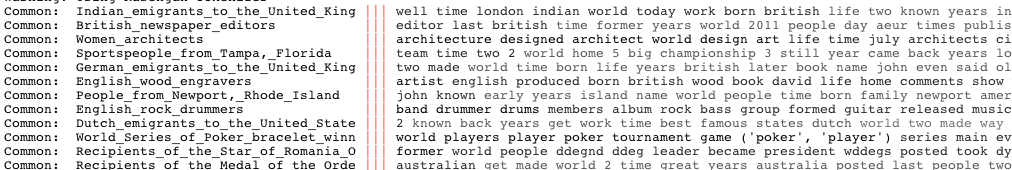
\includegraphics[width=1.18\linewidth]{figures/feature_analysis.png}
  \caption{Naive Bayes Top Features}
  \label{fig:nb-feature-analysis}
\end{adjustwidth}
\end{figure}

We show the performance of this method on the
\textit{catpeople-dev} dataset.
\begin{table}[htbp]
  \centering
\rowcolors{1}{}{lightgrey}
  \begin{tabular}{r  c  c c }\toprule
                 & Feature Selection (Top 20\%) & Feature Selection (Top 70\%) & Feature Selection (Top 60\%) \\
MA-AUPR          & 0.034                        & 0.206                        & 0.197                        \\
MA-Rand-AUPR     & 0.013                        & 0.015                        & 0.013                        \\
MA-P-Top10       & 0.203                        & 1.513                        & 1.487                        \\
MA-P-Top10-Rand  & 0.073                        & 0.073                        & 0.073                        \\
MA-P-Top100      & 1.550                        & 4.453                        & 4.557                        \\
MA-P-Top100-Rand & 0.767                        & 0.843                        & 0.780                        \\
MA-MRR           & 0.094                        & 0.385                        & 0.358                        \\
MA-Rand-MRR      & 0.009                        & 0.009                        & 0.009                        \\
\bottomrule\end{tabular}
  \caption{print 100\% Training. 100 Categories from Dev data.}
  \label{tab:summary-nb}
\end{table}

It is illustrative to perform a deeper error analysis.
We can see that some of the categories perform quite well with just this
heuristic while others do not.
We analyzed the category of \verb|Indian_emigrants_to_the_United_Kingdom| in
detail and found the following two sources of errors.
\begin{enumerate}
\item The descriptive features were not present in the text. For example, the
  entity \verb|Anurag_Dikshit| does not have features like \textit{british},
  \textit{uk}. Instead he lives in \textit{Gibraltar} which is a british
  principality. Essentially the relevant feature was missing.
  We call this the \textit{type 1} error.
\item Wrong descriptive features were chosen from the example entities.
  We call the prescence of noisy features \textit{type 2} errors.
\item The descriptive features were erroneously present in the text for the wrong
  entities. For example, the entity \textit{Nina\_Sudden} contains the words
  \textit{indian}, and \textit{british} even though she is not indian. These are
  \textit{type 3} errors.
\end{enumerate}
In the paper \verb|recovery.tex| we analyse \textit{type 1, 2} errors.

\begin{table}[htbp]
  \centering
  \begin{tabular}{l | c  | c }\toprule
\verb|Indian_emigrants_to_the_United_Kingdom    |          & 0.013 0.002 & 0.039 0.010 \\
\verb|British_newspaper_editors                 |          & 0.048 0.030 & 0.017 0.001 \\
\verb|Women_architects                          |          & 0.188 0.110 & 0.013 0.005 \\
\verb|Sportspeople_from_Tampa,_Florida          |          & 0.089 0.062 & 0.031 0.004 \\
\verb|German_emigrants_to_the_United_Kingdom    |          & 0.024 0.002 & 0.043 0.009 \\
\verb|English_wood_engravers                    |          & 0.081 0.056 & 0.024 0.011 \\
\verb|People_from_Newport,_Rhode_Island         |          & 0.021 0.002 & 0.034 0.010 \\
\bullet{\verb|English_rock_drummers             |}         & 0.455 0.041 & 0.085 0.029 \\
\verb|Dutch_emigrants_to_the_United_States      |          & 0.029 0.015 & 0.042 0.010 \\
\bullet{\verb|World_Series_of_Poker_bracelet_winners    |} & 0.946 0.024 & 0.043 0.022 \\
\bottomrule\end{tabular}
  \caption{print 100\% Training, Feat\_select=Features that occur in 80\% of the document}
  \label{tab:feat-select-doc-80}
\end{table}

Given the above results and the above analysis, how can we reduce each of these
three types of errors?
\begin{description}
\item[Type 1 Error] Requires a very notion of query expansion which in turn
  requires a notion of word similarity. We can
  incorporate methods like feature expansion based on PPDB, or $k$-nn type
  methods based on a metric between; a set of bag of vectors and a bag of
  vectors.
\item[Type 2 Error] We need to discard some of the features that are present in
  the entities, even though they may be present in all of the examples.
  Essentially requires a prior on the types
  of features that can possibly be useful, which in turn requires a prior on the
  types of queries that can be performed. This is hard to do automatically and
  requires human intervention. Simple methods like stop-word removal, and
  keeping only those features that appear in a specified percentage of the
  entities are useful but what should one do if the wrong feature is present in
  all of the entities?
\item[Type 3 Error] Two approaches can be used to reduce such errors.
  First, better feature engineering can
  reduce these errors. For example, instead of using only tokens one can use
  tuples of features and dependency parses, that should reduce the false
  occurrence of descriptive features in the wrong entities. Of course changing
  the feature representation in this way can increase the type 1 errors, but it
  should decrease the type 2 errors as well.

  The second method is to

  A third method is to use a supervised learning technique such as learning to
  rank and then to learn the weights of features that are conjunctions of the
  original features. Or to learn \textit{VETO} features and to use them through
  a \textit{cascade of classifiers} based approach. Of course once we move to
  the supervised approach then various possibilities open up. Such as learning
  to rank through boosted decision trees, which incidentally has been done by
  Chris Burges as the McRank method.
  ``Learning to Rank Using Classification and Gradient Boosting''\\
  ``McRank: Learning to Rank Using Multiple Classification and Gradient
  Boosting''\\
  Tatikonda, S. and Parthasarathy, S. (2011) ``Mining Tree-Structured Data on
  Multicore Systems'', in Bekkerman, R., Bilenko, M., and Langford, J. (eds.)
  Scaling up Machine Learning: Parallel and Distributed Approaches. Cambridge
  University Press, pp. 420–445.
\end{description}



% \begin{table}[htbp]
%   \centering
%   \begin{tabular}{l | c | c}\toprule
% \verb|Indian_emigrants_to_the_United_Kingdom    | & 0.101 0.047 & 0.022 0.005 \\
% \verb|British_newspaper_editors                 | & 0.084 0.079 & 0.036 0.025 \\
% \verb|Women_architects                          | & 0.059 0.021 & 0.014 0.001 \\
% \verb|Sportspeople_from_Tampa,_Florida          | & 0.083 0.035 & 0.025 0.006 \\
% \verb|German_emigrants_to_the_United_Kingdom    | & 0.066 0.044 & 0.040 0.005 \\
% \verb|English_wood_engravers                    | & 0.169 0.049 & 0.012 0.001 \\
% \verb|People_from_Newport,_Rhode_Island         | & 0.086 0.053 & 0.026 0.007 \\
% \bullet{\verb|English_rock_drummers                     |}  & 0.503 0.031 & 0.062 0.005 \\
% \verb|Dutch_emigrants_to_the_United_States      | & 0.065 0.037 & 0.035 0.004 \\
% \bullet{\verb|World_Series_of_Poker_bracelet_winners    |} & 0.899 0.033 & 0.047 0.027 \\
%     \bottomrule\end{tabular}
%   \caption{Print $100\%$ Training, Feat\_select=top20}
%   \label{tab:nb1}
% \end{table}

% \begin{table}[htbp]
%   \centering
%   \begin{tabular}{l | c | c }\toprule
% \verb|Indian_emigrants_to_the_United_Kingdom    | & 0.073 0.030 & 0.075 0.071 \\
% \verb|British_newspaper_editors                 | & 0.045 0.019 & 0.049 0.027 \\
% \verb|Women_architects                          | & 0.039 0.011 & 0.026 0.006 \\
% \verb|Sportspeople_from_Tampa,_Florida          | & 0.068 0.017 & 0.040 0.021 \\
% \verb|German_emigrants_to_the_United_Kingdom    | & 0.060 0.037 & 0.037 0.019 \\
% \verb|English_wood_engravers                    | & 0.066 0.043 & 0.016 0.007 \\
% \verb|People_from_Newport,_Rhode_Island         | & 0.050 0.025 & 0.041 0.031 \\
% \bullet{\verb|English_rock_drummers                     |} & 0.488 0.014 & 0.075 0.010 \\
% \verb|Dutch_emigrants_to_the_United_States      | & 0.045 0.012 & 0.029 0.002 \\
% \bullet{\verb|World_Series_of_Poker_bracelet_winners    |} & 0.777 0.075 & 0.027 0.006 \\
%     \bottomrule\end{tabular}
%   \caption{Print 50\% Training, Feat\_select=top20}
%   \label{tab:nb2}
% \end{table}

\section{To Do}
\label{sec:todo}
\begin{enumerate}
\item I promised results with extra metrics.
\item I promised experiments using kernel based aproach.
\item I promised experiments using a leraning to rank appraoch.
\item I promised to scale up the experiments.
\item I promised eperiments where I discover the common concept first and did
  the reranking based on the common concepts.
\item I promised that I wil add IDF to the reranking score.
\end{enumerate}


\section{Discussion}
\label{sec:discussion}

\bibliographystyle{abbrv}
\bibliography{references}
\end{document}
